% !TeX encoding = UTF-8
% !TeX spellcheck = en_US

\documentclass[
	ruledheaders=chapter,
	class=report,
	thesis={type=master, department=inf},
	accentcolor=1c,
	custommargins=true,
	marginpar=false,
	parskip=half-,
	fontsize=11pt,
]{tudapub}

\usepackage[english]{babel}

\usepackage[autostyle]{csquotes}
\usepackage{microtype}

\usepackage{enumerate}
\usepackage{enumitem}

\usepackage{biblatex}
\bibliography{thesis-literature}

\usepackage{tabularx}
\usepackage{booktabs}

\usepackage{mathtools}
\usepackage{amssymb}

\usepackage{graphicx}
\usepackage{float}
\usepackage[export]{adjustbox}
\usepackage[font=small,labelfont=bf]{caption}
\graphicspath{ {./images/} }

\counterwithout{footnote}{chapter}

\pagenumbering{roman}

\begin{document}
	\Metadata{
		title=Evaluating the Efficacy of Gaussian Padding on Website Fingerprinting Attacks,
		author=Johannes Leupold
	}
	
	\title{Evaluating the Efficacy of Gaussian Padding on Website Fingerprinting Attacks}
	\author[J. Leupold]{Johannes Leupold}
	\birthplace{Dresden}
	\reviewer{Jean-Paul Degabriele \and Vukasin Karadzic}

	\department{inf}
	\institute{IT Security}
	\group{Cryptography and Network Security}
	
	\submissiondate{01.09.2021}
	\examdate{20.09.2021}
	
	% Hinweis zur Lizenz:
	% TUDa-CI verwendet momentan die Lizenz CC BY-NC-ND 2.0 DE als Voreinstellung.
	% Die TU Darmstadt hat jedoch die Empfehlung von dieser auf die liberalere
	% CC BY 4.0 geändert. Diese erlaubt eine Verwendung bearbeiteter Versionen und
	% die kommerzielle Nutzung.
	% TUDa-CI wird im nächsten größeren Release ebenfalls diese Anpassung vornehmen.
	% Aus diesem Grund wird empfohlen die Lizenz manuell auszuwählen.
	% \tuprints{urn=1234,printid=12345,doi=10.25534/tuprints-1234,license=cc-by-4.0}
	% To see furhter information on the license option in English, remove the license= key and pay attention to the warning & help message.
	
	% \dedication{Für alle, die \TeX{} nutzen.}
	
	\maketitle
	
	\affidavit[digital]% oder \affidavit[digital] falls eine rein digitale Abgabe vorgesehen ist.

	\begin{abstract}[english]
		Abstract
	\end{abstract}
	
	\tableofcontents
	
	\chapter{Introduction}
	\label{introduction}
	\IMRADlabel{introduction}
	\pagenumbering{arabic}

	This is the introduction.

	\chapter{Background Material}
	\label{fingerprinting}

	\section{Theoretical Setting}
	\label{theoretical}
	
	Website Fingerprinting (WF) is a field of study focusing on data leaked from anonymization 
	techniques and whether it is still sufficient to conclude which websites the user visited.
	Furthermore, a goal of Website Fingerprinting study is the evaluation of various countermeasures
	that limit the leaked data and thus thwart attempts to uncover the websites a certain user was
	visiting.
	
	\subsection{Threat Model}
	\label{theoretical:threat_model}
	
	The Website Fingerprinting adversary is assumed to have access to the encrypted network traffic of the victim. However, he is not able to decrypt the traffic, or parts of it, so he can only draw conclusions based on metadata of the encrypted packets. In particular, the adversary observes 
	
	\begin{itemize}
		\item packet length (full packet size in bytes),
		\item direction (whether the packet goes from Client $\to$ Server, or vice versa), and
		\item timing (amount of time between the first packet and the current packet).
	\end{itemize}

	This information also gives way to various derived measures, such as overall bandwidth consumed, overall time, or burst\footnote{A \textit{burst} is a contiguous sequence of packets going in the same direction} length/size.
	
	Before the adversary begins with the attack, he can create a database of websites the victim may visit and collect so-called \textit{packet traces} for the websites. A packet trace is a sequence $\mathcal{T} = \langle p_1,p_2,...,p_n\rangle$ of tuples $p_i = (t_i, l_i, d_i) \in \mathbb{N} \times \{52, \ldots, MTU\} \times \{\uparrow, \downarrow\}, i = 1,\ldots,n$, where $t_i$, $l_i$ and $d_i$ denote the time, length and direction for a single observed packet, respectively. The packet length can never be smaller than 52 bytes, as that is the size of the smallest possible TCP/IP packet, the ACK packet. The maximum packet size $MTU$ (also called \textit{Maximum Transmission Unit}) is dependent on the used network technologies. For Ethernet, the MTU is 1500 bytes, while for WiFi (IEEE 802.11) it is 2312 bytes. Note that the adversary is assumed to collect his database of website traces under the same technical preconditions (network technologies) that his victim uses to access them. When carrying out the attack, the adversary observes packet traces for particular page loads of the victim. He may then use any algorithm and his prepared database to try and deduce which websites out of the pre-selected set the victim visited. When a WF countermeasure is in place, the adversary is assumed to be aware of it such that he can collect his trace database under the same countermeasure.
	
	WF threats may be considered either in the Closed World or the Open world scenario. In the Closed World, the goal of the adversary is to identify the websites a victim visited from a fixed set of websites known in advance, while in the Open World scenario, the adversary defines a set of monitored web pages and intends to identify whether the victim visited a website from that set.
	
	
	\subsection{Attacks}
	\label{theoretical:attacks}
	
	To successfully make conclusions on the websites a victim visited, the attacker needs to classify the packet traces he observed to be an instance of one of the websites in his database. He may achieve this by randomly guessing the instance's class, but this naive method can't be expected to yield good results for higher numbers of websites. Therefore, the adversary may employ a Machine Learning technique, consisting of a feature extraction\footnote{\textit{Feature Extraction} refers to transforming a certain observation into a number of (mostly numerical) attributes, called \textit{features}} and a classification algorithm. A classification algorithm is trained using a number of examples from all classes including the class labels (the \textit{training set}). In the following, an overview of common classification algorithms is given.
	
	\subsubsection{Nearest Neighbors}
	\label{ml:nn}
	
	The Nearest Neighbors classifier (also called NN) is a simple algorithm that assigns to each instance the class of its nearest neighbor according to some distance metric. It may be extended to $k$-Nearest-Neighbors ($k$-NN) by considering the nearest $k$ neighbors and taking the majority vote of their classes. One may also apply weighting to the neighbors based on the distance from the point to be classified. The NN classifier is an instance of $k$-NN for $k = 1$.
	
	\textbf{Training:} The NN classifier is trained using a number of data points and their respective classes, which it stores internally. Also, a distance metric is selected.
	
	\textbf{Classification:} Being presented a data point, the $k$-NN classifier looks for the closest $k$ neighbors of the point among its stored training points with respect to the chosen distance metric. It then returns the class label which the majority of those neighbors have.
		
	\subsubsection{Naive Bayes} 
	
	The Naive Bayes classifier tries to estimate probability distributions for the attribute values conditioned on all classes from the training data. To classify a new example, Bayes' rule is used to calculate the conditional probability of the example for each class $C$ and the class yielding the highest probability is returned.
	
	\textbf{Training:} The NB classifier is trained using a number of data points and their respective classes. It may estimate the prior probability of the classes $p(C)$ from their relative frequency in the data or use a predefined prior (e.g. uniform). Then it estimates a conditional probability distribution on data attributes $p(x \mid C)$ for every class $C$. This may be done by fitting a normal distribution to the data using a maximum likelihood estimate (or any other probability distribution that is considered to fit the data), or by employing Kernel Density Estimation (see below). 
	
	\textbf{Classification:} To classify a new data point $x$, the NB classifier uses Bayes' rule to calculate the conditional probability of each class given the point:
	
	\begin{align*}
		p(C \mid x) &= \frac{p(x \mid C) \cdot p(C)}{p(x)}
		\intertext{The probabilities $p(C)$ and $p(x \mid C)$ are known due to the training. $p(x)$, the total probability of point $x$, is the same for all classes, hence the following proportionality holds}
		p(C \mid x) &\propto p(x \mid C) \cdot p(C)
	\end{align*}

	After calculating $p(x \mid C) \cdot p(C)$ for all classes $C$, the NB classifier returns the class that yields the highest such value.
	
	\paragraph{Kernel Density Estimation (KDE)} The term "Kernel Density Estimation" refers to a method used to estimate the underlying probability density function a certain set of samples was drawn from. As opposed to maximum likelihood methods that require the distribution's type to be known in advance, KDE is able to approximate any probability distribution. The accuracy of this approximation depends in large parts on the smoothing parameter $h$, called the \textit{bandwidth}, which controls the area of influence a single data point has on the resulting probability density. See Figure \ref{fig:kde} for an example. When evaluating the estimated density function at a certain point, a so-called \textit{kernel} function is centered over each training sample, and evaluated to obtain the probability density. A kernel is a non-negative function, which is usually chosen to be symmetric and centered on zero\footnote{Most of the time, the kernel should itself be a probability density, leading the estimated density to be a valid probability density as well}. A common choice is the standard normal distribution, although there are many other options as well\footnote{See \url{https://scikit-learn.org/stable/modules/density.html}, Section 2.8.2 for a non-exhaustive list}.
	
	\begin{figure}[tb]
		\centering
		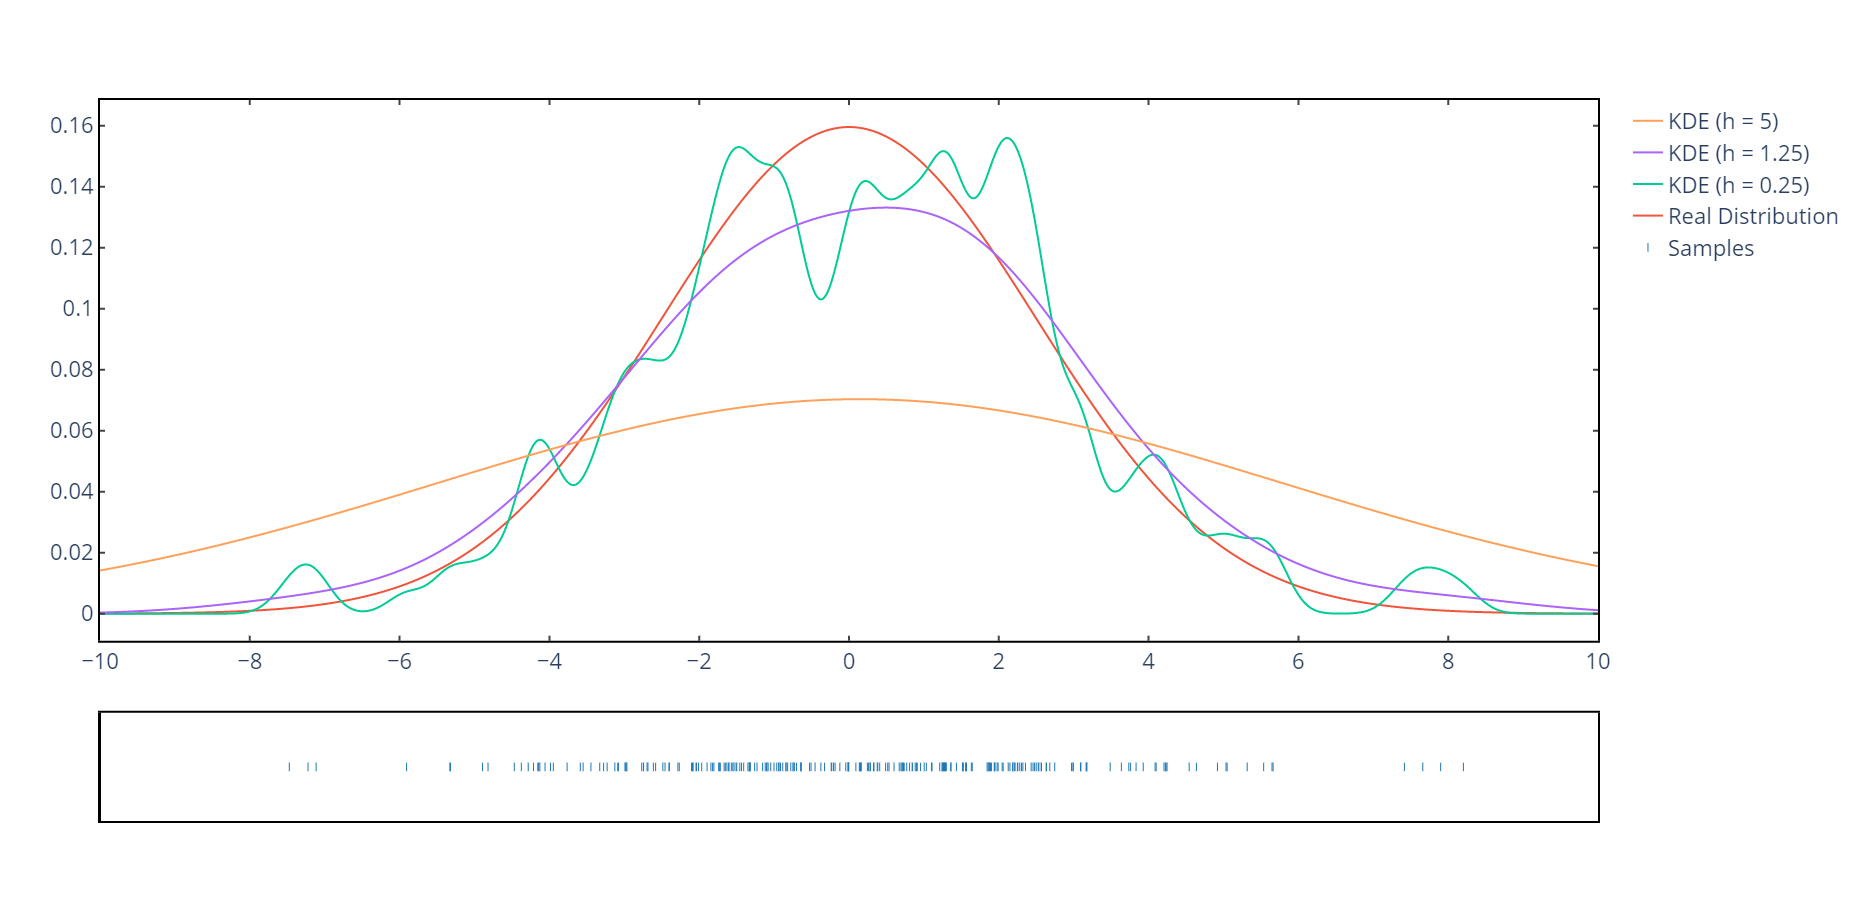
\includegraphics[width=\textwidth]{kde.png}
		\caption{Result of applying KDE with different bandwidths, real distribution and samples are shown}
		\label{fig:kde}
	\end{figure} 

	\textbf{Training:} The Kernel Density Estimator is trained with a number of samples that are stored internally. Additionally, a kernel is selected.
	
	\textbf{Estimation:} To estimate the density at a certain point $x$, the individual centered kernels for every training example $x_i$ are evaluated at the point $x$. Subsequently, the results are summed and scaled to get valid probability values. Equation \ref{eq:kde} shows the full formula.
	
	\begin{equation}
		\label{eq:kde}
		p(x) = \frac{1}{nh}\sum_{i = 1}^{n} k\left(\frac{x - x_i}{h}\right)
	\end{equation}
		
	\subsubsection{Support Vector Machine (SVM)} 
	
	The SVM is a sophisticated classification algorithm trying learn a hyperplane to separate the examples of different classes in the feature space. This is achieved by selecting the hyperplane that yields the largest separation between the classes, i.e. the one that maximizes the distance (the \textit{margin}) to the nearest points of each class. Intuitively, this leads to a better generalization ability to unseen examples, as class separation is maximal. Support Vector Machines are well suited for working with high-dimensional feature spaces and may use a non-linear transformation of data points into an implicit higher-dimensional (and even infinite-dimensional) feature space. This transformation is called a \textit{kernel} (not to be confused with the kernel used in Kernel Density Estimation). An advantage of SVMs is the possibility of sparse representation, as only training examples on, within, or on the wrong side of the margin, called \textit{support vectors}, need to be retained for constructing the hyperplane. A cost parameter $C$ penalizes support vectors that are inside the margin or on the wrong side of the hyperplane. See Figure \ref{fig:svm} for an example. \cite{Boser1992,Cortes1995}.
	
	\begin{figure}[tb]
		\centering
		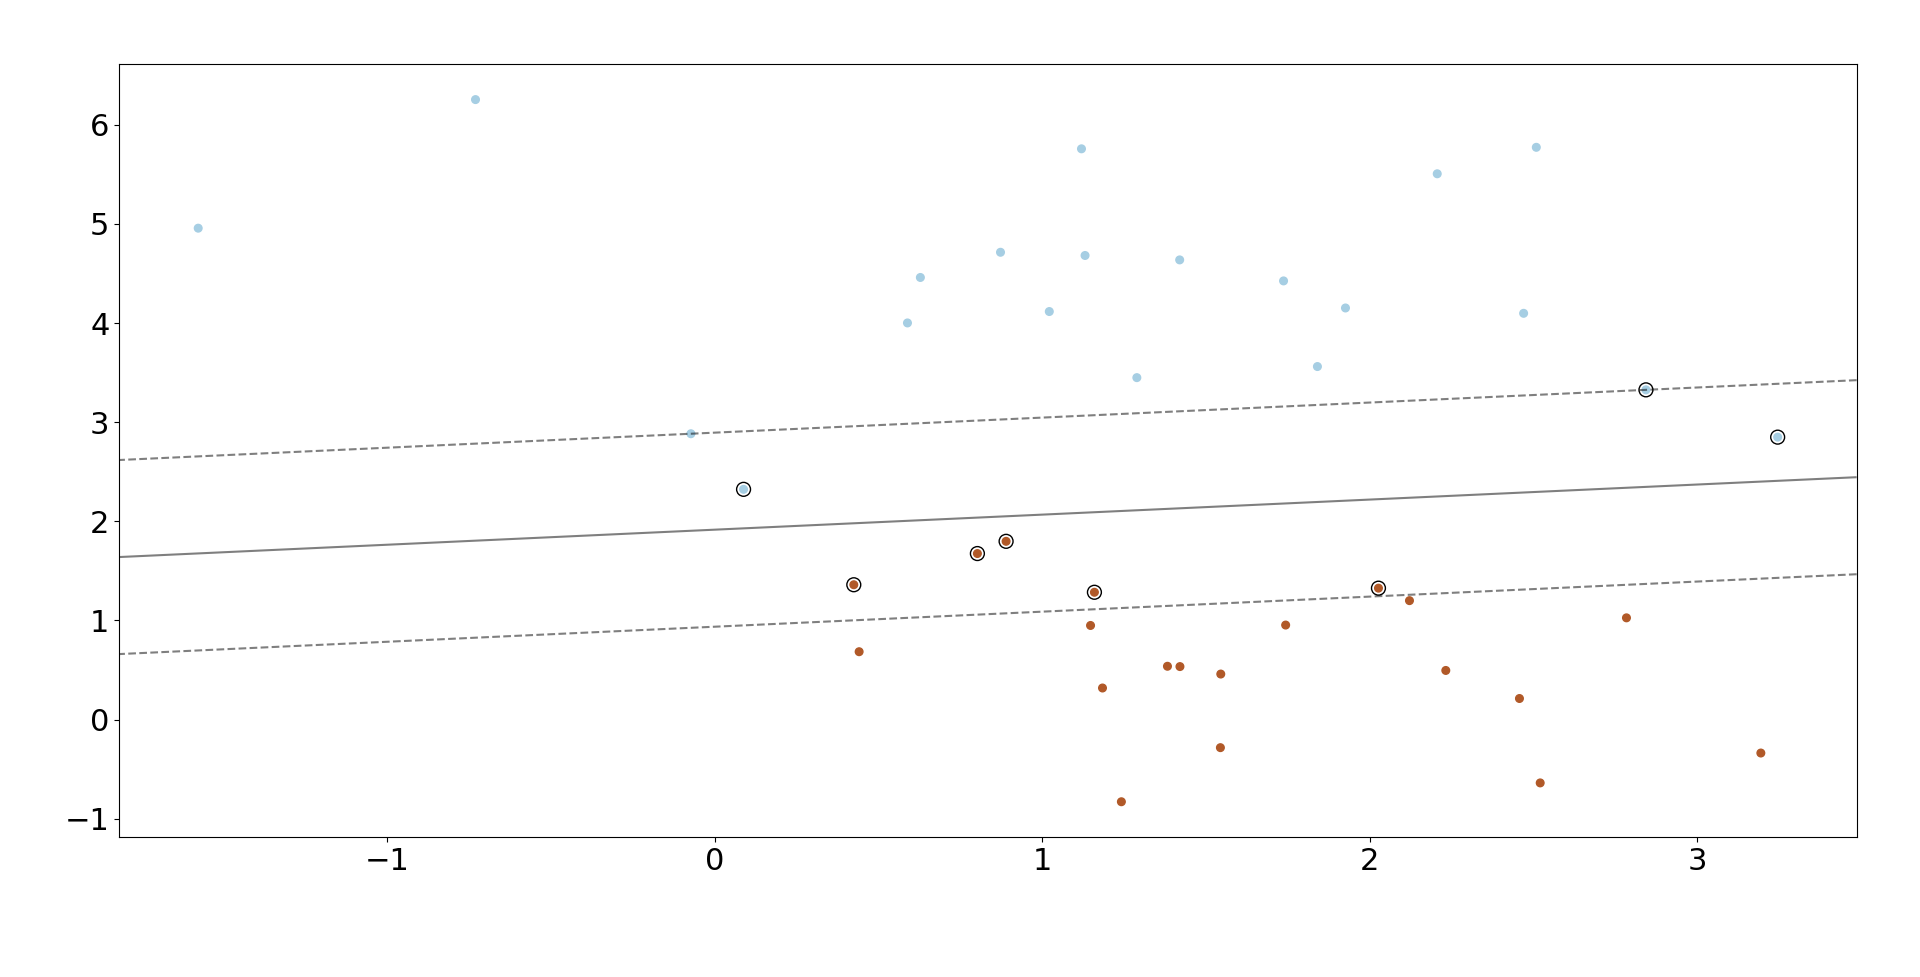
\includegraphics[width=\textwidth]{svm.png}
		\caption{The decision surface of a SVM (with $C = 1$), shown in solid gray and the margin (shown in dashed gray). Training examples are colored by their class, while support vectors are outlined by a black circle (taken from \cite{sklearn-linearSvc} with modifications).}
		\label{fig:svm}
	\end{figure}

	\textbf{Training:} During training, the SVM solves the optimization problem of finding the hyperplane that best separates the data while maximizing the margin. This is done with respect to the penalty parameter $C$. The training examples on or within the margin and on the wrong side of the hyperplane are designated as support vectors. All other training examples may be deleted.
	
	\textbf{Classification:} The separating hyperplane is fully defined given the support vectors. After reconstructing the hyperplane, the example is assigned a class according to on which side of the hyperplane it lies.

	\subsection{Countermeasures}
	\label{theoretical:defenses}

	A defense against WF attacks aims at disguising the identifying patterns in the packet traces the attacker can observe. To this end, packets lengths may be artificially changed, they may be split up into multiple packets, or the timing might be changed. There exist three main classes of defenses, while, naturally, some countermeasures might not fit one particular class, but exhibit characteristics of multiple classes.
	
	\begin{description}
		\item[Padding] Padding schemes are among the simplest countermeasures. They add certain amounts of dummy data to each packet up to the MTU. Padding schemes may be \textit{deterministic} or \textit{probabilistic}, with deterministic schemes always returning the same output trace when presented the same input trace, while this isn't the case for probabilistic padding. When using this type of defense, packets can only grow, but never shrink. Also, packet counts and timing are not affected.
		\item[Noise] Defenses of this class try to disguise the visited web page by deliberately adding noise to the transmission. This can be done for example by loading a second randomly chosen web site in parallel to the requested site \cite{Panchenko2011} or randomizing the order of HTTP requests in the web browser \cite{Perry2011}. Countermeasures using approach may affect packet timing and order and insert new packets into the trace.
		\item[Morphing] Morphing countermeasures are the most complex defenses, trying to hide the actual distribution of packet sizes. They may simply try to make all websites look equal, or at least similar, (cf. \cite{Dyer2012,Cai2014,Cai2014a}) or to make a certain web site look like a different one \cite{Wright2009}. Packet traces may be changed in many ways when using a morphing defense, like adding extra packets, growing or splitting packets, or changing timing.
	\end{description}
	
	\section{Gaussian Padding}
	\label{gaussian_padding}
	
	\textit{Gaussian padding} is a specific form of probabilistic padding. The amount of dummy data added to a packet is drawn from a rounded normal distribution, as opposed to Uniform Padding, where padding sizes are drawn according to the uniform distribution. Furthermore, the tails of the distribution are clipped on both sides, as padding can never take negative values and packets may never become bigger than the MTU. The distribution is parameterized with the desired mean padding size, becoming the mean $\mu$ of the normal distribution. The standard deviation $\sigma$ can be chosen such that the truncated tail corresponds to as little probability mass as desired. For our purpose, choosing $\sigma = \frac{\mu}{3}$ is sufficient, as in this case only approximately $0.1\%$ of the probability mass is allocated to negative values. Figure \ref{fig:trunc_gauss} shows an example distribution function for a truncated rounded normal distribution.
	
	Sampling from a rounded normal distribution is straight-forward by simply sampling from a continuous normal distribution and rounding the value. The truncation can be achieved by rejecting and resampling values that fall out of the desired interval, or by using the method described by Hülsing et al. in \cite{Huelsing2018}, which allows to sample from a rounded Gaussian in constant time, thus mitigating cache timing attacks on the sampling algorithm. While these are out of scope under the threat model of WF, this fact is of particular interest for different fields of research, such as Lattice-based cryptography. \cite{Huelsing2018}
	
	When applying Gaussian padding, the amount of data added to each packet may either be sampled from the distribution independently for each individual packet or once for every session (i.e. page load), leading to \textit{packet-random} Gaussian padding and \textit{session-random} Gaussian padding, respectively.
	
	\begin{figure}[tb]
		\centering
		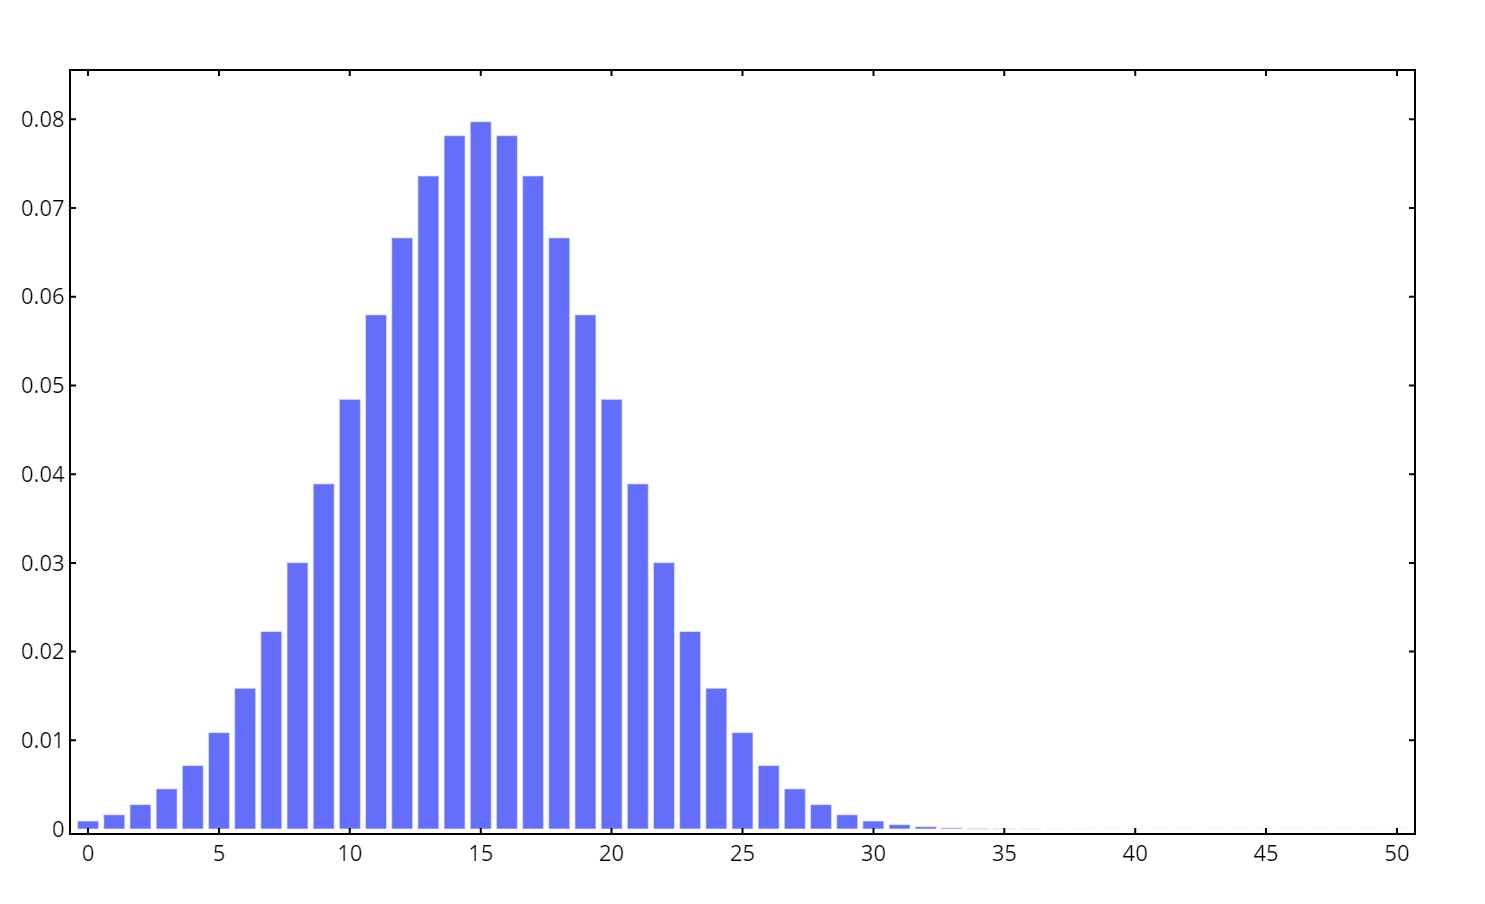
\includegraphics[width=\textwidth]{truncated_rounded_normal.png}
		\caption{An example for a rounded normal distribution, truncated to the left at 0 with a mean padding size of $\mu = 15$ and a standard deviation of $\sigma = 5$ }
		\label{fig:trunc_gauss}
	\end{figure}

	\chapter{Prior Work}
	\label{prior}
	
	Website fingerprinting attacks and defenses have been subject to an "arms race which has continued for more than a decade" \cite{Cherubin2017}. In the following sections, a selection of major WF attacks (Section \ref{prior:attacks}) and defenses (Section \ref{prior:defenses}) are presented. Furthermore, Section \ref{prior:cherubin_bounds} gives an overview over a method proposed by Cherubin \cite{Cherubin2017} to estimate provable security bounds for WF defenses with respect to a given feature set.
	
	\section{Website Fingerprinting Attacks}
	\label{prior:attacks}
	
	Many WF attacks have been published during the last 15 years, with each one improving on the accuracy and performance (including robustness against countermeasures) of the previous attacks. A selection of notable such attacks is presented below, in order of increasing recency. While the early publications still focused on fingerprinting encrypted traffic on SSH tunnels (cf. \cite{Liberatore2006,Herrmann2009,Panchenko2011,Dyer2012}), with the rise in popularity of the Tor anonymization platform\footnote{\url{https://www.torproject.org/}} the focus in the WF community has since shifted heavily towards Tor traffic in the recent years (cf. \cite{Dyer2012,Wang2014,Panchenko2016,Hayes2016,Sirinam2018,Wang2021}). Tor traces pose additional challenges to the attacker, as in Tor all packets have equal length and some countermeasures have already been deployed \cite{Perry2011}. Starting from the \textit{H} attack below, all subsequent attacks are increasingly focused on Tor, with everything beyond \textit{VNG++} no longer considering SSH traffic at all.
	
	\paragraph{LL} In \cite{Liberatore2006}, Liberatore and Levine present two distinct attacks, one based on a modified Jaccard coefficient (a measure for set similarity), and a second one using a Naive Bayes classifier with KDE. While both attacks have been found to yield good results, the Jaccard classifier's accuracy degrades more rapidly in the face of countermeasures \cite{Liberatore2006}. Because of this, most of subsequent work only considered the Naive Bayes classifier, which will be termed \textit{LL} going forward. The attack of Liberatore and Levine uses as features a histogram of packet sizes and directions, i.e. counting the numbers of packets having each size going in each direction. Apart from their contributions to WF attacks, Liberatore and Levine have also published a dataset of website traces for WF evaluation (see Section \ref{methods:dataset} for more details).
	
	\paragraph{H} The attack by Herrmann et al. \cite{Herrmann2009} uses the same feature set as the LL attack, but instead of using the Naive Bayes classifier, it applies a set of well-known text mining transformations on the packet size histogram, namely the \textit{TF (term frequency) transformation} (equation \ref{eq:tf}) and \textit{cosine normalization} (equation \ref{eq:cosine}). Then, they apply the Multinomial Naive Bayes classifier, which is commonly used in text mining \cite{Herrmann2009}. A detailed description of the classifier can be found in \cite[ch. 13]{Manning2008}.
	
	\begin{flalign}
		f^*_{x_i} &= log(1 + f_{x_i}) \label{eq:tf} \\
		\intertext{The $x_i$ values denote pairs of packet directions and sizes $(d, l) \in \{\uparrow,\downarrow\} \times \{52, \ldots, MTU\}$, while $f_{x_i}$ is the absolute frequency of such packets in the trace. Below, $\|\cdot\|$ denotes the euclidean norm.}
		f^{norm}_{x_i} &= \frac{f^*_i}{\left\| (f^*_{x_1}, \ldots, f^*_{x_m}) \right\| } \label{eq:cosine}
	\end{flalign}

	\paragraph{P} A very impactful attack was proposed by Panchenko et al. in \cite{Panchenko2011}. It was one of the first attacks to consider also some coarse-grained features in addition to packet histograms. In particular, information about overall bandwidth, count of distinct packet sizes, fraction of upstream/downstream packets and bursts are added to the feature set. Additionally, they employ a SVM for classification. Altogether, their attack reaches very high accuracy (more than 96\% for 775 websites) even for high class (or, website) counts and has been found robust to many countermeasures \cite{Dyer2012}.
	
	\paragraph{VNG++} In their work in \cite{Dyer2012}, Dyer et al. not only present a comprehensive survey on existing WF attacks and defenses, but also explore the feasibility of website fingerprinting without using a packet histogram, as all previous attacks had been doing. They find that, when using only the overall upload and download bandwidth, the total transmission time and a burst size histogram, results similar to that of the P attack can be achieved while using a Naive Bayes classifier with KDE. Dyer et al. also note that, using the same feature set as the P attack, but the NB classifier instead of a SVM, performance doesn't degrade much from the original P attack, suggesting that using a complex classification algorithm isn't necessary to obtain good results in WF \cite{Dyer2012}.
	
	\paragraph{$k$-NN} Wang et al. \cite{Wang2014} further developed the idea of using a simple classification algorithm by resorting to the $k$-NN classifier and choosing a large set of different features, including total bandwidth and transmission time, occurrence of unique packet sizes, information on packet ordering and bursts (although with a slightly different definition than the one that was given earlier) as well as the size and direction of the first 20 packets in each trace. Furthermore, they determine weights for all features signifying their relative importance, which are multiplied with the feature vectors prior to classification. For the detailed description of the algorithms, refer to \cite{Wang2014}.
	
	\paragraph{CUMUL} A more recent contribution of Panchenko et al. \cite{Panchenko2016}, the CUMUL attack also uses a SVM classifier, like the P attack did before. While Wang et al. used a multitude of manually selected features in their $k$-NN attack (up to 4000), Panchenko et al. focus on creating an abstract representation that implicitly covers the characteristics of a page load \cite{Wang2014,Panchenko2016}. In addition to the basic features of packet count and bandwidth per direction, they create a cumulative sum of the packet sequence (with outgoing packets having negative size) and sample a fixed number $n$ of additional features from this cumulative sum using linear interpolation. In their work, Panchenko et al. find $n = 100$ to yield good results, leading to only 104 features in total \cite{Panchenko2016}.
	
	\paragraph{Recent Attacks} Many more attacks have been published in recent years which are mentioned here for the sake of completeness. Hayes and Danezis published the $k$-FP (or $k$-Fingerprinting) attack where they are using a modified Random Forest classifier to extract an abstract fingerprint for each website, which is then classified using the $k$-NN classifier \cite{Hayes2016}. Sirinam et al. employ deep learning techniques, namely Convolutional Neural Networks (CNN), to website fingerprinting, yielding the DF (Deep Fingerprinting) attack \cite{Sirinam2018}. Later, Wang et al. proposed the Adaptive Fingerprinting (AF) attack, greatly reducing the amount of data needed to train the deep learning algorithms\footnote{Usually, deep learning algorithms require a very large amount of training data due to their complex nature and slow optimization convergence}. At the same time, AF reduces the need to frequently update the training data due to the sensitivity to content changes of contained websites \cite{Wang2021}.
	
	\section{Website Fingerprinting Defenses}
	\label{prior:defenses}
	
	In the following, a number of major WF defenses from all the three classes (cf. Section \ref{theoretical:defenses}) will be briefly presented.
	
	\paragraph{Classical Padding Defenses} There are a multitude of padding schemes that can be applied to the WF setting, some of which are deterministic and some probabilistic. A good overview of them is given in \cite{Dyer2012}. Table \ref{tbl:padding} also shows a selection of them.
	
	\begin{table}
		\centering
		\small
		\begin{tabularx}{\textwidth}{|l|l|X|}
			\hline \textbf{Name} & \textbf{Type} & \textbf{Description} \\
			\hline Linear Padding & deterministic & pad to the next multiple of 128 bytes, or the MTU \\
			\hline Exponential Padding & deterministic & pad to the next power of two, or the MTU \\
			\hline Mice-Elephants & deterministic & pad to 128 bytes if the packet has $l \leq 128$, or otherwise to the MTU \\
			\hline Pad to MTU & deterministic & Each packet size is increased to the MTU \\
			\hline 
			\hline Session Random 255 & probabilistic & Sample a value $r \in \{0, 8, 16, ..., 248\}$ uniformly at random for the session. Increase each packet length by this amount. \\
			\hline Packet Random 255 & probabilistic & Sample a value $r \in \{0, 8, 16, ..., 248\}$ uniformly at random for each packet. Increase the packet length by this amount. \\
			\hline
		\end{tabularx}
		\caption{An overview of classical padding schemes that have been applied to website fingerprinting \cite{Dyer2012}}
		\label{tbl:padding}
	\end{table}

	\paragraph{Defense by Noise} Several defenses using noise to disguise a website's identifying patterns have been proposed in the past. One notable examples are \textit{Decoy Pages}, as proposed by Panchenko et al. in \cite{Panchenko2011}, where a random webpage is loaded in parallel to the desired web page, thus producing noise through unrelated traffic. Another such defense is \textit{Randomized Pipelining}, as deployed in the Tor Browser, which randomizes the order of parallel HTTP requests sent over the same connection (HTTP pipelining) \cite{Perry2011,Cherubin2017}.
	
	\paragraph{Morphing Defenses} One of the first publications studying morphing defenses is the \textit{Traffic Morphing} algorithm by Wright et al. \cite{Wright2009}. This defense tries to make web pages look like other pages by learning a so-called \textit{morphing matrix} that transforms the packet size distribution (\textit{source distribution}) such that it resembles the distribution of a different web page (\textit{target distribution}). The morphing matrix is learned using convex optimization to maximize the similarity between the source and target distributions while keeping the overhead minimal. During the process, packets may be split and resized to match the target distribution best. Another similar algorithm presented by Dyer et al. in \cite{Dyer2012} is called \textit{Direct Target Sampling}, where the complex morphing step is skipped and target packet sizes are sampled directly from the selected target distribution.
	
	Another class of morphing defenses aims at reducing differences between the traces of different websites, thus making it harder to distinguish them. They try to limit information available to the attacker. Examples for such defenses are shown in Table \ref{tbl:morphing}.
	
	\begin{table}
		\centering
		\begin{tabularx}{\textwidth}{|l|l|X|}
			\hline \textbf{Name} & \textbf{Authors} & \textbf{Description} \\
			\hline BuFLO & Dyer et al. \cite{Dyer2012} & Sends packets of fixed size $d$ at a fixed interval $\rho$ for at least a fixed time $\tau$, introducing dummy packets when needed \\
			\hline Tamaraw & Cai et al. \cite{Cai2014} & Sends packets of fixed size $d$ at fixed intervals, while the interval $\rho_{out}$ for outgoing packets and $\rho_{in}$ for incoming packets are distinct and $\rho_{out} > \rho_{in}$. Pads the number of packets in either direction by multiples of a parameter. \cite{Cherubin2017} \\
			\hline CS-BuFLO & Cai et al. \cite{Cai2014a} & Similar to BuFLO, but adapts $\rho$ to the available network bandwidth dynamically. \\
			\hline
		\end{tabularx}
		\caption{Examples for morphing defenses trying to reduce information available to the attacker}
		\label{tbl:morphing}
	\end{table}
			
	\section[Security Bound Estimation]{Security Bound Estimation According to Cherubin \cite{Cherubin2017}}
	\label{prior:cherubin_bounds}
	
	When evaluating WF attacks and defenses, the traditional approach is to empirically measure their performance on a previously collected data set of packet traces. However, such empirical
	evaluations are susceptible to noise and fail to produce provable statements on the security of
	a certain defense. While a defense may perform particularly well against the attacks it is evaluated on, it may just as well horribly fail on a different attack that wasn't considered yet. To address this problem and further advance research on provable security evaluation of WF defenses, Cherubin introduces a novel method centered around the Bayes error in \cite{Cherubin2017}.
	
	The \textit{Bayes error} is defined as the minimum probability of error that any classifier can commit given a joint probability distribution on the features and class labels.  Intuitively speaking, the Bayes error corresponds to the area of uncertainty in the probability distribution, i.e. the area where the conditional probabilities $p(x \mid c_i)$ and $p(x \mid c_j)$ overlap\footnote{That is, both probabilities are non-zero} for any two classes $c_i \neq c_j$ and features $x$. 
	
	To formalize, let $\mathcal{X}$ be the feature space and $\mathcal{C}$ the set of all class labels. Let $p(x, c)$ be a joint probability distribution on $\mathcal{X}\times\mathcal{C}$. Then for the set of classifiers $\mathcal{F} = \{f \mid f : \mathcal{X} \to \mathcal{C}\}$ with $R_f$ being the error of a classifier $f\in\mathcal{F}$ according to $p$, the Bayes error $R^*$ is defined as
	
	\begin{align}
		R^* &= \min_{f\in\mathcal{F}} R_f
		\intertext{This minimum error is achieved by the \textit{Bayes classifier} $f^*\in\mathcal{F}$ that assigns to each example $x$ the class label $c$ maximizing the probability $p(c \mid x)$ \cite{Duda2000}.}
		f^*(x) &= \arg\max_{c\in\mathcal{C}} p(c \mid x) \\
		R^* &= R_{f^*}
	\end{align}
	
	As the true joint probability distribution $p(x, c)$ is typically not known in practice, the exact value of the Bayes error can't be calculated. However, there are well-known methods to estimate a lower bound for the Bayes error. Cherubin uses an estimate based on the NN classifier (see Section \ref{ml:nn}) first presented by Cover and Hart \cite{Cover1967} deriving a lower bound $\widehat{R}^*$ for the Bayes error $R^*$
	
	\begin{equation}
		\widehat{R}^* = \frac{L - 1}{L} \left(1 - \sqrt{1 - \frac{L}{L-1}\widehat{R}_{NN}}\right) \leq R^*
	\end{equation}
	
	where $\widehat{R}_{NN}$ is the empirical error of the NN classifier on a data set containing $L = |\mathcal{C}|$ classes.

	\chapter{Experimental Methodology}
	\label{methods}
	\IMRADlabel{methods}

	\section{Trace Data}
	\label{methods:dataset}

	\section{Evaluating Attack Performance}
	\label{pipeline}

	\section{Error Bound Estimation}
	\label{error_bound_estimation}

	\chapter{Results}
	\label{results}
	\IMRADlabel{results}

	\section{Empirical Performance of Gaussian Padding}
	\label{performance}

	\section{Estimated Security Bounds}
	\label{security_bounds}

	\chapter{Discussion}
	\label{discussion}
	\IMRADlabel{discussion}

	\chapter{Conclusion}
	\label{conclusion}

	\pagebreak
	\pagenumbering{roman}
	\setcounter{page}{5}
	\addcontentsline{toc}{chapter}{Bibliography}
	\printbibliography

	\cleardoublepage
	\phantomsection
	\addcontentsline{toc}{chapter}{\listfigurename}
	\listoffigures

	\cleardoublepage
	\phantomsection
	\addcontentsline{toc}{chapter}{\listtablename}
	\listoftables
\end{document}